%\section{Experiments}
We test our methods for reducing bias amplification in two problem settings: visual semantic role labeling in the imSitu dataset (vSRL) and multilabel image classification in MS-COCO (MLC). 
In all settings we derive corpus constraints using the training set and then run our calibration method in batch on either the development or testing set. 
Our results are summarized in Table~\ref{tab:results} and Figure~\ref{fig:results}.
%using two different settings:  \textit{batch} setting and \textit{online} setting. 
%In batch setting, we have access to all the test instances. 
%Therefore, we can calibrate the gender ratio on them. 
%We show this result on the dev set. In online setting, we only can access one instance at a time. 
%Therefore, we cannot add corpus-wise constraints. 
%However, we show that we can still remove the amplified biases in such test instance by applying the offset we obtained from the batch setting.
% We get the lambdas using the training and dev dataset and then adopt it to the test dataset. Besides trying to remove gender bias, we also test our \alg again on the verb bias issue, because we notice that for some verbs like ``fixing'' are more likely to appear when the system detects there is a man  in the image.
\subsection{Visual Semantic Role Labeling}
Our quantitative results are summarized in the first two sections of Table~\ref{tab:results}.
On the development set, the number of verbs whose bias exceed the original bias by over 5\% decreases 30.5\% (Viol.).
Overall, we are able to significantly reduce bias amplification in vSRL by 52\% on the development set (Amp. bias).
We evaluate the underlying recognition performance using the standard measure in vSRL:  top-1 semantic role accuracy, which tests how often the correct verb was predicted and the noun value was correctly assigned to a semantic role.
Our calibration method results in a negligible decrease in performance (Perf.).
In Figure~\ref{fig:gender_ratio_afterLR} we can see that the overall distance to the training set distribution after applying \alg{} decreased significantly, over 39\%. 


\begin{table}[t]
\centering
    \begin{tabular}{|l|c|c|c|}
 
        \hline
         \bf Method & \bf Viol. & \bf Amp. bias & \bf Perf. (\%) \\
         \hline
          \multicolumn{4}{|c|}{vSRL: Development Set} \\
          \hline
        CRF  &  154   & 0.050  & 24.07 \\
         \hline
        CRF + \alg &  107 & 0.024  & 23.97\\
        \hline
        \multicolumn{4}{|c|}{vSRL: Test Set} \\
        \hline
        CRF  &  149   & 0.042 & 24.14 \\
         \hline
        CRF + \alg &  102 & 0.025 & 24.01\\
        \hline
          \multicolumn{4}{|c|}{MLC: Development Set} \\
          \hline
     CRF  &  40   & 0.032  & 45.27 \\
         \hline
        CRF + \alg &  24 & 0.022  & 45.19\\
        \hline
    \multicolumn{4}{|c|}{MLC: Test Set} \\
         \hline
          CRF  &  38   & 0.040  &  45.40\\
         \hline
        CRF + \alg &  16 & 0.021  & 45.38\\
        \hline
    \end{tabular}
    \caption{
    Number of violated constraints, mean amplified bias, and test performance before and after calibration using \alg{}. 
    The test performances of vSRL and MLC are measured by top-1 semantic role accuracy and  top-1 mean average precision, respectively.}
    \label{tab:results}
\end{table}

\begin{figure*}[!h]
    \centering
    % \hspace{-30pt}
       \begin{subfigure}[b]{0.49\textwidth}
        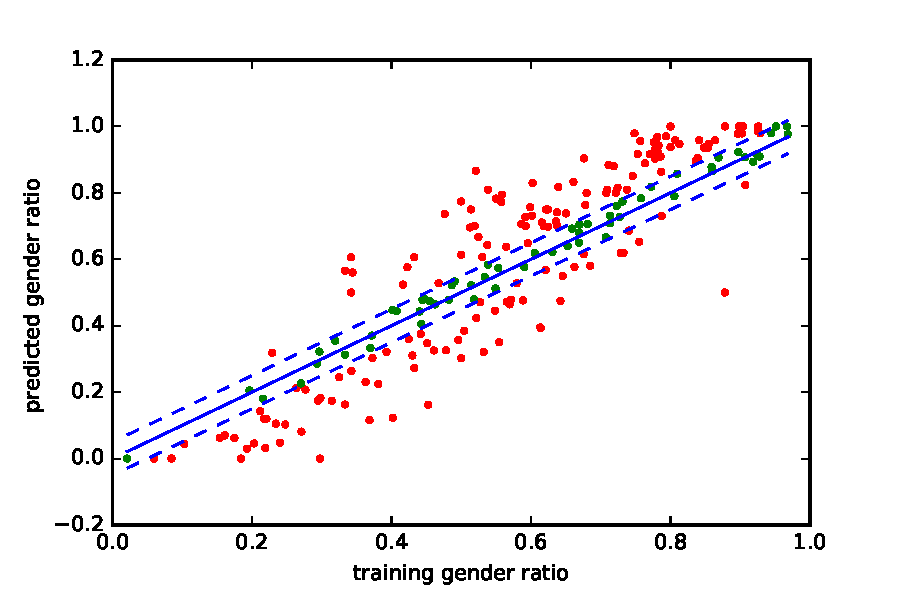
\includegraphics[width=1.1\linewidth]{figures/train_x/imSitu_gender_ratio_tx_dev005_beforeLR.pdf}
        \caption{Bias analysis on imSitu vSRL without \alg}
        \label{fig:gender_ratio_beforeLR}
    \end{subfigure}
    %   \hspace{-16pt}
    \begin{subfigure}[b]{0.49\textwidth}
        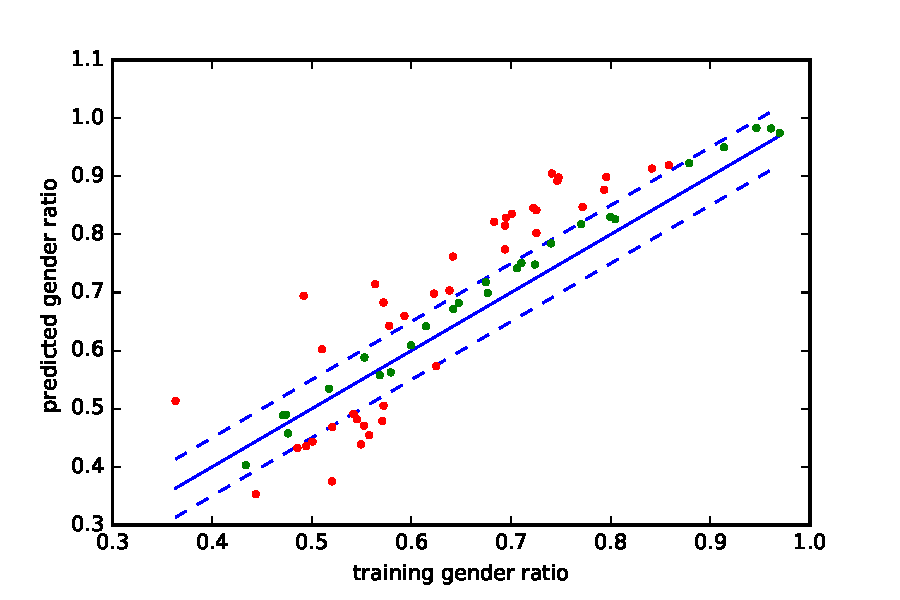
\includegraphics[width=1.1\linewidth]{figures/train_x/coco_gender_ratio_005_beforeLR.pdf}
        \caption{Bias analysis on MS-COCO MLC without \alg}
        \label{fig:coco_gender_ratio_beforeLR}
    \end{subfigure}
      \vspace{10pt}
    %   \hspace{-16pt}    
      \begin{subfigure}[b]{0.49\textwidth}
        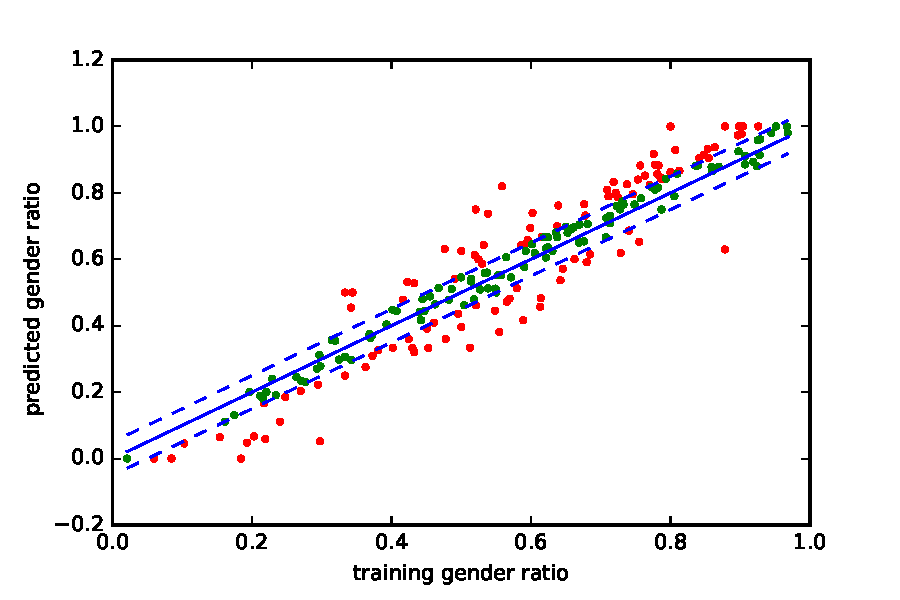
\includegraphics[width=1.1\linewidth]{figures/train_x/imSitu_gender_ratio_tx_dev005_afterLR.pdf}
        \caption{Bias analysis on imSitu vSRL with \alg }
        \label{fig:gender_ratio_afterLR}
    \end{subfigure}
    \begin{subfigure}[b]{0.49\textwidth}
        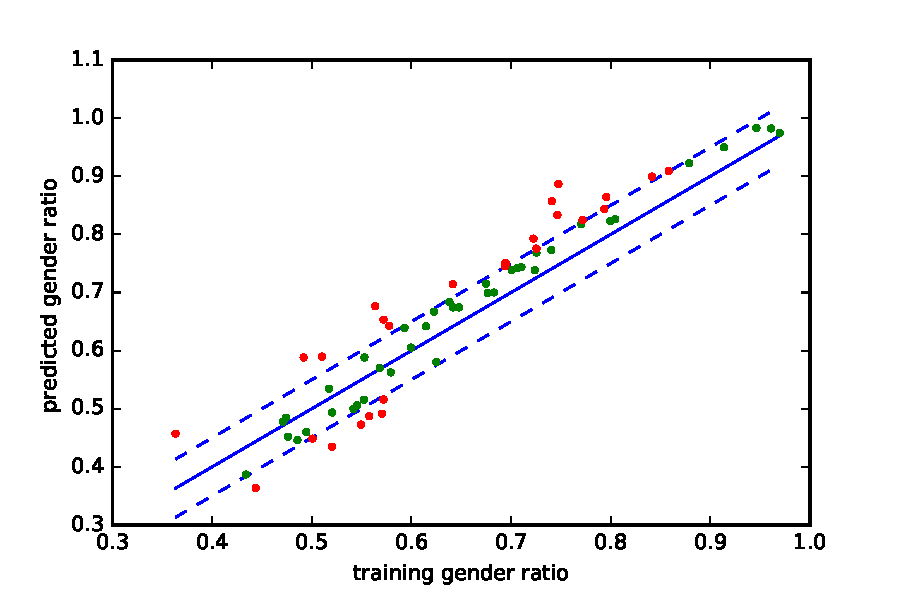
\includegraphics[width=1.1\linewidth]{figures/train_x/coco_gender_ratio_005_afterLR.pdf}
        \caption{Bias analysis on MS-COCO MLC with \alg }
        \label{fig:coco_gender_ratio_afterLR}
    \end{subfigure}
      \vspace{10pt}
    \begin{subfigure}[b]{0.49\textwidth}
        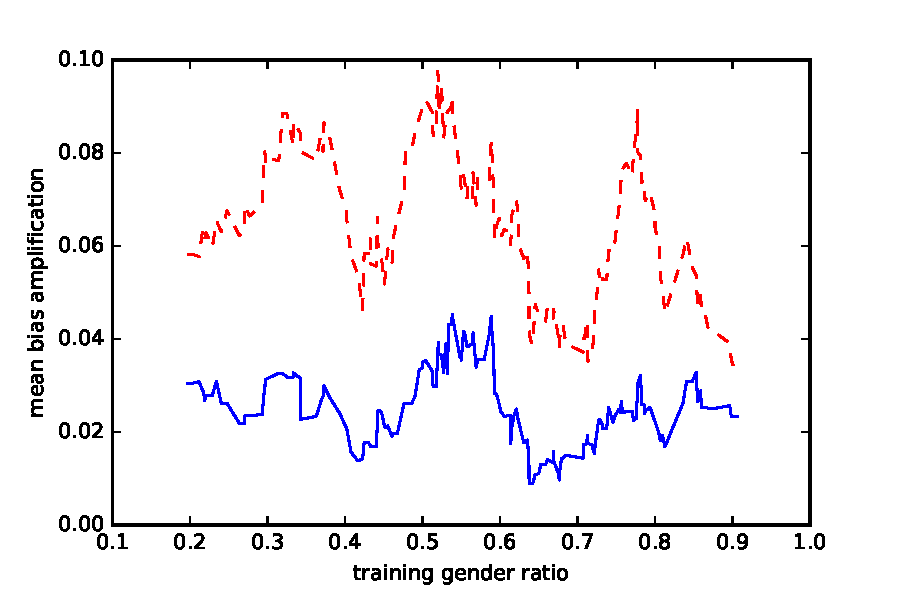
\includegraphics[width=1.1\linewidth]{figures/train_x/imSitu_mean_gender_ratio_dis_tx_dev_005.pdf}
        \caption{Bias in vSRL with (blue) / without (red) \alg}
        \label{fig:mean_gender_ratio_dis}
    \end{subfigure}    
    \begin{subfigure}[b]{0.49\textwidth}
        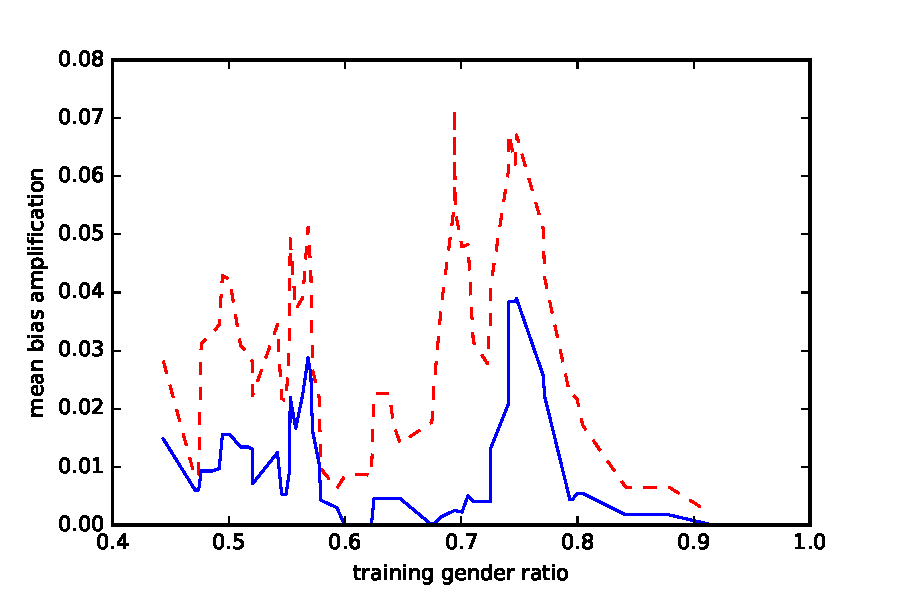
\includegraphics[width=1.1\linewidth]{figures/train_x/coco_mean_gender_ratio_dis_tx_dev_005.pdf}
        \caption{Bias in MLC with (blue) / without (red) \alg}
        \label{fig:coco_mean_gender_ratio_dis}
    \end{subfigure}
    \caption{
    Results of reducing bias amplification using \alg on imSitu vSRL and MS-COCO MLC.
    Figures 3(a)-(d) show initial training set bias along the x-axis and development set bias along the y-axis. 
    Dotted blue lines indicate the $0.05$ margin used in \alg, with points violating the margin shown in red while points meeting the margin are shown in green. 
    Across both settings adding \alg significantly reduces the number of violations, and reduces the bias amplification significantly. 
    Figures 3(e)-(f) demonstrate bias amplification as a function of training bias, with and without \alg. 
    Across all initial training biases, \alg  is able to reduce the bias amplification.
    } 
    \label{fig:results}
\end{figure*}


Figure~\ref{fig:mean_gender_ratio_dis} demonstrates that across all initial training bias, \alg{} is able to reduce bias amplification. 
In general, \alg{} struggles to remove bias amplification in areas of low initial training bias, likely because bias is encoded in image statistics and cannot be removed as effectively with an image agnostic adjustment.
Results on the test set support our development set results: we decrease bias amplification by 40.5\% (Amp. bias).
\subsection{Multilabel Classification}
Our quantitative results on MS-COCO RBA are summarized in the last two sections of Table~\ref{tab:results}. 
Similarly to vSRL, we are able to reduce the number of objects whose bias exceeds the original training bias by 5\%, by 40\% (Viol.).
Bias amplification was reduced by 31.3\% on the development set (Amp. bias). 
The underlying recognition system was evaluated by the standard measure: top-1 mean average precision, the precision averaged across object categories.
Our calibration method results in a negligible loss in performance.
In Figure~\ref{fig:coco_gender_ratio_afterLR}, we demonstrate that we substantially reduce the distance between training bias and bias in the development set.
Finally, in Figure~\ref{fig:coco_mean_gender_ratio_dis} we demonstrate that we decrease bias amplification for all initial training bias settings. 
Results on the test set support our development results: we decrease bias amplification by 47.5\% (Amp. bias).
\subsection{Discussion}
We have demonstrated that \alg{} can significantly reduce bias amplification.
While were not able to remove all amplification, we have made significant progress with little or no loss in underlying recognition performance. 
Across both problems, \alg{} was able to reduce bias amplification at all initial values of training bias. 


%\subsection{Experiments for Gender Ratio}
%\label{sec:gender_ratio}

%In this section, we will set the constraints to the verbs to say that the predicted gender ratio should be within the margin of the gender ratio in training dataset.
%For this experiment, we only consider 212 human-related verbs.
%All of these 212 verbs have more than 50 times with either a ``man'' or ``woman'' as the agent and in the prediction, more than 20 times ``man'' or ``woman'' occurs as its agent. 
% Here we set the margin to be $0.05$ 
% is because that about $91.5\%$ of the verbs in batch setting are within this margin of the training dataset (reference). 
%We here set the margin to $0.05$ but in practice, the margin can be assigned to any reasonable value. \jy{we also have some results about another margins which will be shown in appendix.} The result is shown in Fig.~\ref{fig:imSitu_gender_ratio}.

%\paragraph{Batch Setting.} 

 %The blue line is the gender ratio we get from the training data, and the dotted blue line is the training ratio $\pm 0.13$. 
% All those violated verbs in prediction are marked with red dots while others are the green ones.
 %From Fig.~\ref{fig:gender_ratio_beforeLR} and~\ref{fig:gender_ratio_afterLR} we can see that after adopting \alg, most of the gender ratio for these verbs are modified to within the margin. 
 %We also shows the mean difference between the predicted gender ratio to the margin for all the verbs in Fig.~\ref{fig:mean_gender_ratio_dis}  showing that \alg  can push the gender ratio closer to the reference.

%\paragraph{Online Setting.}

%When doing the predictions, sometimes we cannot get access to the ground truth. 
%However with the results on batch setting, we can still remove the amplified bias in some sense. 
%The results are shown in  Fig.~\ref{fig:test_gender_ratio_beforeLR} to~\ref{fig:test_mean_gender_ratio_dis}. 
%Even though we do not know the ground truth, we can still help to reduce the amplified bias with the  result from the batch setting.
%We also get the statistics for the results in Table~\ref{tab:gender_ratio_number}. $Mv$ %stands for number of violated verbs.  
%$Dt$ is the difference of gender ratio between prediction and ground-truth for all verbs.
%$Acc$ is the top-1 accuracy for all the semantic role-value pair predictions. 
%We can see that \alg{} can help to reduce the gender bias while has very little affect on %the accuracy of the system.

% \begin{table}
% \centering
%     \begin{tabular}{@{ }c@{ }|@{ }c@{ }|@{ }c@{ }|@{ }c@{ }|@{ }c@{ }|@{ }c@{ }|@{ }c@{ }}
%     % \hline
%         \bf     &  \bf Tv   &  \bf Mv  &  \bf Dm & \bf Dt1 & \bf Dt2 & \bf Acc \\ \hline
%         n-\alg-dev  & 221 &  147  &   4.23 & 22.09 & 12.69 & 0.2407\\
%         \alg-dev    & 221 &  168  &  1.85 & 19.09 & 7.57 &  0.2401\\
%         n-\alg-test  & 221 &  142 &   4.68 & 22.31 & 13.77 & 0.2413\\
%         \alg-test    & 221 &  157 &  3.99 & 21.14 & 11.15 & 0.2411\\
%     \end{tabular}
%     \caption{Statistic results for removing gender bias with or without our \alg.}
%     \label{tab:gender_ratio_number}
% \end{table}

%\begin{table}
%\centering
    %\begin{tabular}{|l|c|c|c|c|}
    %     Method & \bf Viol.  & \bf Mean Dist & \bf Ampl & \bf \overline{Acc} \\
    %     \hline
    %    CRF  &  154  &  10.41 & 5.02  & 24.07 \\
    %     \hline
    %    CRF + \alg &  106  & 6.33 & 2.39  & 23.97\\
    %    \hline
    %\end{tabular}
    %\caption{
    %Results on vSRL before and calibration. Viol is the number margin violating verbs, %distance is the average distance to the training ratio, bias amplification is the %mean  
    %Statistic results for gender bias with or without our \alg. $Mv$ is the number of  %verbs out of margin.  $Dt$ is the gender ratio distance from ground-truth for all %verbs. $Acc$ is the top-1 accuracy for all the semantic role-value pairs.}
%    \label{tab:gender_ratio_number}
%\end{table}

\iffalse
\begin{table}[t]
\centering
    \begin{tabular}{|l|c|c|c|c|}
         \hline
         Method & \bf Viol. & \bf Amp. bias & \bf mAP  \\
         \hline
        CRF  &  40   & 0.032  & 45.27 \\
         \hline
        CRF + \alg &  27 & 0.023  & 45.22\\
        \hline
    \end{tabular}
    \caption{
    Number of margin violations, mean amplified bias, and MLC top-1 mean average precision before and after calibration with \alg on the MS-COCO development set.}
    \label{tab:gender_ratio_number}
\end{table}

\begin{table}[t]
\centering
    \begin{tabular}{|l|c|c|c|c|}
         \hline
         Method & \bf Viol. & \bf Amp. bias & \bf mAP  \\
         \hline
        CRF  &  39   & 0.036  &  45.40\\
         \hline
        CRF + \alg &  20 & 0.024  & 45.37\\
        \hline
    \end{tabular}
    \caption{
    Number of margin violations, mean amplified bias, and MLC top-1 mean average precision before and after calibration with \alg on the MS-COCO test set.}
    \label{tab:gender_ratio_number}
\end{table}

\fi

%0.0499 --> 0.0265

\iffalse
\begin{table}[t]
\centering
    \begin{tabular}{|l|c|c|c|c|}
         \hline
         Method & \bf Viol. & \bf Amp. bias & \bf arg-acc \\
         \hline
        CRF  &  141   & .049 &24.13 \\
         \hline
        CRF + \alg &  97 & .027 & 24.00\\
        \hline
    \end{tabular}
    \caption{
    Number of margin violations, mean amplified bias, and vSRL top-1 semantic role accuracy before and after calibration with \alg on the imSitu testing set.}
    \label{tab:gender_ratio_number}
\end{table}

\fi

%\jy{report distance on dev dataset compared to dev gold ratio}
% \begin{figure*}[!h]
%     \centering
%     \hspace{-30pt}
%       \begin{subfigure}[b]{0.25\textwidth}
%         \includegraphics[width=\linewidth]{figures/imSitu_gender_ratio_dis_to_dev_50_013_01_beforeLR.pdf}
%         \caption{Gender ratio difference between predictions on dev and ground truth in dev without LR.}
%         \label{fig:gender_ratio_beforeLR}
%     \end{subfigure}
%     %   \hspace{-16pt}
%     \begin{subfigure}[b]{0.25\textwidth}
%         \includegraphics[width=\linewidth]{figures/imSitu_gender_ratio_dis_to_dev_50_013_01_afterLR.pdf}
%         \caption{Gender ratio difference between predictions on dev and ground truth in dev with LR. }
%         \label{fig:gender_ratio_afterLR}
%     \end{subfigure}
% \end{figure*}


%\paragraph{Batch Setting.} 
%Fig.~\ref{fig:man_dev_verb_ratio_beforeLR} to \ref{fig:man_dev_mean_verb_ratio} are the results on batch setting for man related verbs while  Fig.~\ref{fig:woman_dev_verb_ratio_beforeLR} to \ref{fig:woman_dev_mean_verb_ratio} are the results for woman. 
%For those  man-related verbs, before adopting \alg, there are 165 verbs out of the margin and this number decreases to 134 with \alg{}, meaning we decrease the amount of bias by 19\%.
%We also calculate the distance of the verb ratio to the ground truth for all verbs.
%After \alg, the distance decreases from 0.27 to 0.20. 
%For ``woman'' related verbs  the number of violated verbs decreases from 156 to 119 with 23.7\% bias removed. The distance to the ground truth for all verbs becomes 0.312 with originally value 0.375.

%\paragraph{Online Setting.}
%Fig.~\ref{fig:man_test_verb_ratio_beforeLR} to~\ref{fig:man_test_mean_verb_ratio} and Fig.~\ref{fig:woman_test_verb_ratio_beforeLR} to~\ref{fig:woman_test_mean_verb_ratio} show the results for ``man'' and ``woman'' related images in the online setting. 
%We can see that after applying our \alg, the ratio is closer to the reference one and the difference between the predicted ratio and the margin shrinks. 
%With our \alg{} in man-related dataset, we decrease the number of violated verbs from 170 to 149 and the distance to the ground truth decreases from 0.28 to 0.21.
%For woman-related dataset, the number of violated verbs becomes 128 which is 20 less than not applying \alg{} and also the distance decreases from 0.32 to 0.24. All the results prove the efficiency of our algorithm \alg{}  in removing the amplified bias.
%We also provide the statistic results in Table~\ref{tab:man_verb_ratio_number}. 

% \begin{table}
% \centering
%     \begin{tabular}{@{ }c@{ }|@{ }c@{ }|@{ }c@{ }|@{ }c@{ }|@{ }c@{ }|@{ }c@{ }|@{ }c@{ }}
%     % \hline
%         \bf     &  \bf Tv   &  \bf Mv  &  \bf Dm & \bf Dt1 & \bf Dt2 & \bf Acc \\ \hline
%         n-\alg-dev  & 331 &  166  &   0.126 & 0.351 & 0.274 & 0.315\\
%         \alg-dev    & 331 &  197  &  0.103 & 0.285 & 0.200 &  0.283\\
%         n-\alg-test  & 331 &  161 &  0.133 & 0.356 & 0.281 & 0.311\\
%         \alg-test    & 331 &  182 &  0.084 & 0.295 & 0.209 & 0.286
%     \end{tabular}
%     \caption{Statistic results for removing verb bias from man related images with or without \alg.}
%     \label{tab:man_verb_ratio_number}
% \end{table}

% \begin{table}
% \centering
%     \begin{tabular}{@{ }c@{ }|@{ }c@{ }|@{ }c@{ }|@{ }c@{ }|@{ }c@{ }|@{ }c@{ }|@{ }c@{ }}
%     % \hline
%         \bf     &  \bf Tv   &  \bf Mv  &  \bf Dm & \bf Dt1 & \bf Dt2 & \bf Acc \\ \hline
%         n-\alg-dev  & 268 &  112  &   0.142 & 0.375 & 0.313 & 0.305\\
%         \alg-dev    & 268 &  149  &  0.111 & 0.312 & 0.234 &  0.273\\
%         n-\alg-test  & 268 &  120 &  0.154 & 0.381 & 0.315 & 0.307\\
%         \alg-test    & 268 &  140 &  0.107 & 0.326 & 0.240 & 0.281
%     \end{tabular}
%     \caption{Statistic results for removing verb bias for woman related images with or without our \alg.}
%     \label{tab:woman_verb_ratio_number}
% \end{table}

% \begin{figure*}[!h]
%     \centering
%       \begin{subfigure}[b]{0.3\textwidth}
%         \includegraphics[width=\linewidth]{figures/train_x/imSitu_man_verb_ratio_tx_dev_beforeLR.pdf}
%         \caption{Man-related verb ratio in batch setting without \alg}
%         \label{fig:man_dev_verb_ratio_beforeLR}
%     \end{subfigure}
%     \begin{subfigure}[b]{0.3\textwidth}
%         \includegraphics[width=\linewidth]{figures/train_x/imSitu_man_verb_ratio_tx_dev_afterLR.pdf}
%         \caption{Man-related verb ratio in batch setting with \alg }
%         \label{fig:man_dev_verb_ratio_afterLR}
%     \end{subfigure}
%     \begin{subfigure}[b]{0.3\textwidth}
%         \includegraphics[width=\linewidth]{figures/train_x/imSitu_man_mean_verb_ratio_tx_dev_03.pdf}
%         \caption{Man-related mean verb ratio difference in batch setting}
%         \label{fig:man_dev_mean_verb_ratio}
%     \end{subfigure}
    
%     \begin{subfigure}[b]{0.3\textwidth}
%         \includegraphics[width=\linewidth]{figures/train_x/imSitu_man_verb_ratio_tx_test_beforeLR.pdf}
%         \caption{Man-related verb ratio in online setting without \alg }
%         \label{fig:man_test_verb_ratio_beforeLR}
%     \end{subfigure}
%     \begin{subfigure}[b]{0.3\textwidth}
%         \includegraphics[width=\linewidth]{figures/train_x/imSitu_man_verb_ratio_tx_test_afterLR.pdf}
%         \caption{Man-related verb ratio in online setting with \alg }
%         \label{fig:man_test_verb_ratio_afterLR}
%     \end{subfigure}
%     \begin{subfigure}[b]{0.3\textwidth}
%         \includegraphics[width=\linewidth]{figures/train_x/imSitu_man_mean_verb_ratio_tx_test_03.pdf}
%         \caption{Man-related mean verb ratio difference in online setting}
%         \label{fig:man_test_mean_verb_ratio}
%     \end{subfigure}
    
%     \begin{subfigure}[b]{0.3\textwidth}
%         \includegraphics[width=\linewidth]{figures/train_x/imSitu_woman_verb_ratio_tx_dev_beforeLR.pdf}
%         \caption{Woman-related verb ratio in batch setting without \alg}
%         \label{fig:woman_dev_verb_ratio_beforeLR}
%     \end{subfigure}
%     \begin{subfigure}[b]{0.3\textwidth}
%         \includegraphics[width=\linewidth]{figures/train_x/imSitu_woman_verb_ratio_tx_dev_afterLR.pdf}
%         \caption{Woman-related verb ratio in batch setting with \alg }
%         \label{fig:woman_dev_verb_ratio_afterLR}
%     \end{subfigure}
%     \begin{subfigure}[b]{0.3\textwidth}
%         \includegraphics[width=\linewidth]{figures/train_x/imSitu_woman_mean_verb_ratio_tx_dev_03.pdf}
%         \caption{Woman-related mean verb ratio difference in batch setting }
%         \label{fig:woman_dev_mean_verb_ratio}
%     \end{subfigure}
    
%     \begin{subfigure}[b]{0.3\textwidth}
%         \includegraphics[width=\linewidth]{figures/train_x/imSitu_woman_verb_ratio_tx_test_beforeLR.pdf}
%         \caption{Woman-related verb ratio in online setting without \alg}
%         \label{fig:woman_test_verb_ratio_beforeLR}
%     \end{subfigure}
%     \begin{subfigure}[b]{0.3\textwidth}
%         \includegraphics[width=\linewidth]{figures/train_x/imSitu_woman_verb_ratio_tx_test_afterLR.pdf}
%         \caption{Woman-related verb ratio in online setting with \alg }
%         \label{fig:woman_test_verb_ratio_afterLR}
%     \end{subfigure}
%     \begin{subfigure}[b]{0.3\textwidth}
%         \includegraphics[width=\linewidth]{figures/train_x/imSitu_woman_mean_verb_ratio_tx_test_03.pdf}
%         \caption{Woman-related mean verb ratio difference in online setting}
%         \label{fig:woman_test_mean_verb_ratio}
%     \end{subfigure}
%     \caption{Verb ratio predicted in the visual SRL system. We set the constraints that the verb ratio   should be within some margin to the training ratio. In the left two columns, the blue line is the reference ratio and the red dots are the verbs violate the margin. For all the images in the last column, the solid blue line is the result after adopting \alg{} while the red dashed line is the result without \alg. We can see that after Lagrangian Relaxation, many of the verbs become satisfied to these constraints.} 
%     \label{fig:imSitu_verb_ratio}
% \end{figure*}
